\begin{table}[p]
   \centering
   \footnotesize
   \renewcommand{\arraystretch}{1.15}
   \begin{tabular}{@{}>{\centering\arraybackslash}m{0.3033\textwidth}>{\centering\arraybackslash}m{0.3033\textwidth}>{\centering\arraybackslash}m{0.3033\textwidth}@{}}
      \hline
      \multicolumn{3}{@{}c@{}}{%
         \begin{tabular}{@{}>{\centering\arraybackslash}m{\dimexpr0.455\textwidth+\tabcolsep\relax}>{\centering\arraybackslash}m{\dimexpr0.455\textwidth+\tabcolsep\relax}@{}}
            $G_5$ & Matriz de adyacencia \\
            \hline
            \noalign{\vspace{6pt}}
            \rule{0pt}{0pt}$\vcenter{\hbox{\resizebox{0.25\textwidth}{!}{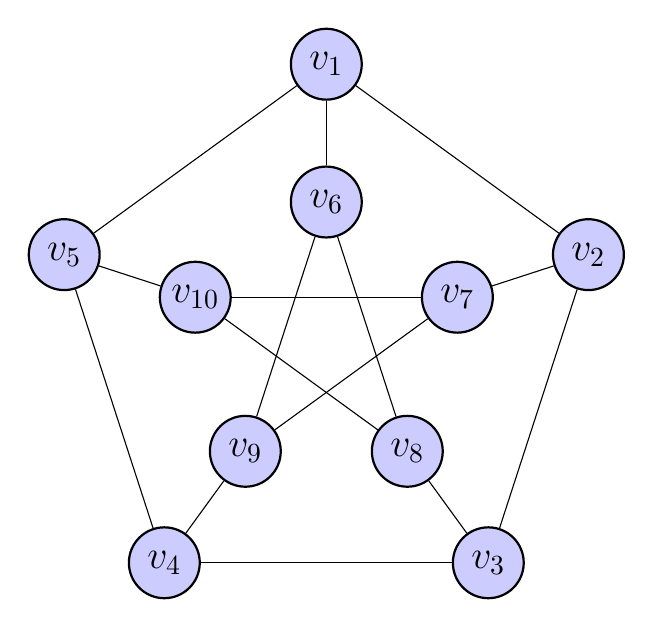
\begin{tikzpicture}[
  scale=1,
  vnode/.style={circle, fill=blue!20, draw=black, thick, minimum size=9mm, inner sep=0pt, font=\Large}
]
  % Vértices del pentágono exterior (en sentido horario desde arriba)
  \node[vnode] (v1) at (90:3.5)  {$v_1$};
  \node[vnode] (v2) at (18:3.5)  {$v_2$};
  \node[vnode] (v3) at (-54:3.5) {$v_3$};
  \node[vnode] (v4) at (-126:3.5) {$v_4$};
  \node[vnode] (v5) at (162:3.5) {$v_5$};

  % Vértices de la estrella interior (en sentido horario desde arriba)
  \node[vnode] (v6)  at (90:1.75)  {$v_6$};
  \node[vnode] (v7)  at (18:1.75)  {$v_7$};
  \node[vnode] (v8)  at (-54:1.75) {$v_8$};
  \node[vnode] (v9)  at (-126:1.75) {$v_9$};
  \node[vnode] (v10) at (162:1.75) {$v_{10}$};

  % Aristas
  \foreach \from/\to in {v1/v2, v2/v3, v3/v4, v4/v5, v5/v1,
                         v1/v6, v2/v7, v3/v8, v4/v9, v5/v10,
                         v6/v8, v8/v10, v10/v7, v7/v9, v9/v6}
    \draw (\from) -- (\to);
\end{tikzpicture}
}}}$
            &
            $\vcenter{\hbox{\tiny$\begin{pmatrix}
         0 & 1 & 0 & 0 & 1 & 1 & 0 & 0 & 0 & 0 \\
         1 & 0 & 1 & 0 & 0 & 0 & 1 & 0 & 0 & 0 \\
         0 & 1 & 0 & 1 & 0 & 0 & 0 & 1 & 0 & 0 \\
         0 & 0 & 1 & 0 & 1 & 0 & 0 & 0 & 1 & 0 \\
         1 & 0 & 0 & 1 & 0 & 0 & 0 & 0 & 0 & 1 \\
         1 & 0 & 0 & 0 & 0 & 0 & 0 & 1 & 1 & 0 \\
         0 & 1 & 0 & 0 & 0 & 0 & 0 & 0 & 1 & 1 \\
         0 & 0 & 1 & 0 & 0 & 1 & 0 & 0 & 0 & 1 \\
         0 & 0 & 0 & 1 & 0 & 1 & 1 & 0 & 0 & 0 \\
         0 & 0 & 0 & 0 & 1 & 0 & 1 & 1 & 0 & 0
      \end{pmatrix}$}}$ \\
            \noalign{\vspace{6pt}}
         \end{tabular}%
      } \\
      \hline
      \multicolumn{3}{c}{\textbf{Topología de adyacencia}} \\
      \hline
      Abiertos subbásicos & Vecindades mínimas & Topología \\
      \hline
         ${A_{v_1}=\{v_2,v_5,v_6\}}$\par
         ${A_{v_2}=\{v_1,v_3,v_7\}}$\par
         ${A_{v_3}=\{v_2,v_4,v_8\}}$\par
         ${A_{v_4}=\{v_3,v_5,v_9\}}$\par
         ${A_{v_5}=\{v_1,v_4,v_{10}\}}$\par
         ${A_{v_6}=\{v_1,v_8,v_9\}}$\par
         ${A_{v_7}=\{v_2,v_9,v_{10}\}}$\par
         ${A_{v_8}=\{v_3,v_6,v_{10}\}}$\par
         ${A_{v_9}=\{v_4,v_6,v_7\}}$\par
         ${A_{v_{10}}=\{v_5,v_7,v_8\}}$
      &
         ${U_{v_1}=\{v_1\}}$\par
         ${U_{v_2}=\{v_2\}}$\par
         ${U_{v_3}=\{v_3\}}$\par
         ${U_{v_4}=\{v_4\}}$\par
         ${U_{v_5}=\{v_5\}}$\par
         ${U_{v_6}=\{v_6\}}$\par
         ${U_{v_7}=\{v_7\}}$\par
         ${U_{v_8}=\{v_8\}}$\par
         ${U_{v_9}=\{v_9\}}$\par
         ${U_{v_{10}}=\{v_{10}\}}$
      &
         $\wp\left(V\left(G_5\right)\right)$ \\[6pt]
      \hline
      \multicolumn{3}{c}{\textbf{Topología de incidencia}} \\
      \hline
      Abiertos subbásicos & Vecindades mínimas & Topología \\
      \hline
         ${e_{1}=\{v_1,v_2\}}$\par
         ${e_{2}=\{v_1,v_5\}}$\par
         ${e_{3}=\{v_1,v_6\}}$\par
         ${e_{4}=\{v_2,v_3\}}$\par
         ${e_{5}=\{v_2,v_7\}}$\par
         ${e_{6}=\{v_3,v_4\}}$\par
         ${e_{7}=\{v_3,v_8\}}$\par
         ${e_{8}=\{v_4,v_5\}}$\par
         ${e_{9}=\{v_4,v_9\}}$\par
         ${e_{10}=\{v_5,v_{10}\}}$\par
         ${e_{11}=\{v_6,v_8\}}$\par
         ${e_{12}=\{v_6,v_9\}}$\par
         ${e_{13}=\{v_7,v_9\}}$\par
         ${e_{14}=\{v_7,v_{10}\}}$\par
         ${e_{15}=\{v_8,v_{10}\}}$
      &
         ${U_{v_1}=\{v_1\}}$\par
         ${U_{v_2}=\{v_2\}}$\par
         ${U_{v_3}=\{v_3\}}$\par
         ${U_{v_4}=\{v_4\}}$\par
         ${U_{v_5}=\{v_5\}}$\par
         ${U_{v_6}=\{v_6\}}$\par
         ${U_{v_7}=\{v_7\}}$\par
         ${U_{v_8}=\{v_8\}}$\par
         ${U_{v_9}=\{v_9\}}$\par
         ${U_{v_{10}}=\{v_{10}\}}$
      &
         $\wp\left(V\left(G_5\right)\right)$ \\[6pt]
      \hline
   \end{tabular}
   \caption{Topologías de adyacencia e incidencia de $G_5$}
   \label{tab:topologias_G_5}

   \vspace{1em}
   \begin{minipage}{\textwidth}
      \normalsize
      El grafo $G_5$ es conocido como \textit{Grafo de Petersen}.
   \end{minipage}
\end{table}
